\documentclass[sigconf,anonymous]{acmart}
\usepackage{amsmath}
\usepackage{booktabs}
\usepackage{tabularx}
\usepackage{balance}
\usepackage{siunitx}
\sisetup{group-minimum-digits=4,group-separator={,}}
\settopmatter{printacmref=false,printfolios=true,printccs=false}
\setlength{\emergencystretch}{1.5em}
\vfuzz=2pt
\setcopyright{none}
\renewcommand\footnotetextcopyrightpermission[1]{}
\acmConference[SIGMOD 2027]{SIGMOD 2027}{Under review}{Anonymous submission}
\acmBooktitle{SIGMOD 2027 Experiments \& Analysis submission}
\acmYear{2027}
\copyrightyear{2027}
\acmDOI{}
\acmISBN{}
\newcommand{\risk}{\mathcal{R}}
\newcommand{\ndc}{\operatorname{NDC}}
\newcommand{\rec}{\operatorname{Recall}}
\newcommand{\indicator}{\mathbf{1}}
\newcommand{\slot}[2]{%
  \fbox{\parbox{\dimexpr\linewidth-2\fboxsep-2\fboxrule\relax}{%
  \small\textbf{Planned exhibit: #1}\par\medskip #2}}}
\newcommand{\sectionaim}[1]{\noindent\textit{Section purpose: #1}\par}

\newcommand{\GraphOnlyRows}{%
hnswlib HNSW & SIFT & 22.31 & 0.77 & 21.55 [20.76, 22.33] & 89.33 \\
Faiss HNSW & SIFT & 23.67 & 0.07 & 23.60 [22.78, 24.39] & 91.07 \\
hnswlib HNSW & Arxiv & 18.24 & 1.07 & 17.17 [16.33, 18.06] & 75.87 \\
Faiss HNSW & Arxiv & 17.93 & 0.17 & 17.77 [16.86, 18.68] & 75.87 \\
}
\newcommand{\RecoveryRows}{%
SIFT & Endpoint & 0.97 [0.53, 1.50] & 0.00 [0.00, 0.00] & 1,826 & 2,615 & 2,855 \\
SIFT & Direct reuse & 6.69 [5.65, 7.77] & 59.51 [57.83, 61.20] & 739 & 2,132 & 2,706 \\
SIFT & Original recalibration & 1.79 [1.25, 2.40] & 44.39 [42.76, 46.01] & 1,015 & 2,349 & 2,774 \\
SIFT & Joint-error replay & 1.79 [1.25, 2.40] & 44.39 [42.76, 46.01] & 1,015 & 2,349 & 2,774 \\
\addlinespace
Arxiv & Endpoint & 1.01 [0.61, 1.47] & 0.00 [0.00, 0.00] & 2,397 & 3,252 & 3,504 \\
Arxiv & Direct reuse & 7.24 [6.18, 8.36] & 64.21 [62.51, 65.85] & 858 & 2,586 & 3,322 \\
Arxiv & Original recalibration & 2.04 [1.45, 2.69] & 44.79 [34.32, 50.96] & 1,323 & 2,974 & 3,398 \\
Arxiv & Joint-error replay & 1.68 [1.10, 2.35] & 29.86 [14.75, 45.00] & 1,681 & 3,117 & 3,460 \\
\addlinespace
}
\newcommand{\CostRows}{%
SIFT & Cached & 129 [129, 129] & 0/10 \\
SIFT & Cold & 396 [395, 397] & 0/10 \\
Arxiv & Cached & 148 [99, 296] & 4/10 \\
Arxiv & Cold & 457 [305, 915] & 4/10 \\
}
\newcommand{\CertificateRows}{%
S & 1103 & 1 & 9 & 3.12 & 3.39 & 2 & 1.44 & C & 1.50 & 44.33 \\
S & 1229 & 1 & 8 & 2.87 & 3.13 & 5 & 2.32 & C & 1.90 & 44.28 \\
S & 1361 & 1 & 10 & 3.37 & 3.65 & 2 & 1.44 & C & 1.80 & 44.29 \\
S & 1499 & 1 & 6 & 2.35 & 2.59 & 3 & 1.74 & C & 2.00 & 44.51 \\
S & 1621 & 1 & 8 & 2.87 & 3.13 & 5 & 2.32 & C & 1.90 & 44.39 \\
S & 1747 & 1 & 11 & 3.62 & 3.90 & 2 & 1.44 & C & 1.90 & 44.28 \\
S & 1877 & 1 & 8 & 2.87 & 3.13 & 4 & 2.04 & C & 1.80 & 44.36 \\
S & 1999 & 1 & 8 & 2.87 & 3.13 & 4 & 2.04 & C & 1.70 & 44.35 \\
S & 2131 & 1 & 6 & 2.35 & 2.59 & 2 & 1.44 & C & 1.70 & 44.53 \\
S & 2267 & 1 & 10 & 3.37 & 3.65 & 2 & 1.44 & C & 1.70 & 44.61 \\
A & 1103 & 1 & 14 & 4.34 & 4.65 & 6 & 2.59 & C & 2.20 & 49.77 \\
A & 1229 & 1 & 17 & 5.06 & 5.39 & 5 & 2.32 & E & 1.30 & 0.00 \\
A & 1361 & 1 & 14 & 4.34 & 4.65 & 3 & 1.74 & C & 2.30 & 49.76 \\
A & 1499 & 1 & 16 & 4.82 & 5.14 & 4 & 2.04 & E & 0.90 & 0.00 \\
A & 1621 & 1 & 16 & 4.82 & 5.14 & 6 & 2.59 & E & 1.10 & 0.00 \\
A & 1747 & 1 & 15 & 4.58 & 4.90 & 6 & 2.59 & C & 1.50 & 49.84 \\
A & 1877 & 1 & 13 & 4.10 & 4.41 & 1 & 1.11 & C & 1.80 & 49.68 \\
A & 1999 & 1 & 13 & 4.10 & 4.41 & 5 & 2.32 & C & 2.20 & 49.80 \\
A & 2131 & 1 & 15 & 4.58 & 4.90 & 5 & 2.32 & C & 2.50 & 49.87 \\
A & 2267 & 1 & 16 & 4.82 & 5.14 & 5 & 2.32 & E & 1.00 & 0.00 \\
}
\newcommand{\SensitivityRows}{%
SIFT & Original & [42.76, 46.01] & [44.33, 44.47] & [42.86, 46.07] \\
SIFT & Joint & [42.76, 46.01] & [44.33, 44.47] & [42.86, 46.07] \\
Arxiv & Original & [34.32, 50.96] & [34.82, 49.81] & [43.27, 46.27] \\
Arxiv & Joint & [14.75, 45.00] & [14.92, 44.80] & [28.85, 30.84] \\
}

% Generated by evidence/check_postseal.py from packaged post-seal evidence.
\newcommand{\TargetCertifiedRows}{%
SIFT & 552/0/0 & 0.126 [0.040, 0.250] & 8.283 [7.921, 8.557] & 0.9964 / 0.9987 & 8.267 \\
Arxiv & 552/0/0 & 0.530 [0.233, 0.915] & 29.083 [28.653, 29.518] & 0.9797 / 0.9828 & 29.027 \\
}
\newcommand{\TargetStageCostRows}{%
SIFT & Pairwise & 552 & 66,914 [64,805, 69,940] & 460 & 100,000 \\
SIFT & Shared target & 24 & 3,019 [2,923, 3,157] & 0 & 10,000 \\
Arxiv & Pairwise & 552 & 17,018 [16,767, 17,276] & 230 & 100,000 \\
Arxiv & Shared target & 24 & 755 [744, 767] & 0 & 1,000 \\
}

\hypersetup{pdfauthor={},pdfsubject={Graph-ANNS budget portability and target recalibration},pdfkeywords={graph ANNS, budget transfer, risk auditing, recalibration}}

\title[Auditing Search-Budget Portability]{Auditing Search-Budget Portability Across Graph-ANNS Rebuilds: [Experiments \& Analysis]}
\author{Anonymous Author(s)}
\begin{document}
\begin{abstract}
Graph indexes are rebuilt to maintain search quality, but the budget policy that serves queries is often retained as reusable state. We study when that policy remains portable, how target evidence should qualify reuse, and when recovery repays its information cost. Across unchanged SIFT-100K and Arxiv-Nomic-100K collections, transferring retrospective first-passing budgets between hnswlib and Faiss builds adds 17.17--23.60 percentage points of query failure relative to target-specific references. After a 5\% data refresh, an unchanged recurring-query policy crosses the 5\% risk limit on both datasets. Index-Conditioned Budget Audit (ICBA) turns these measurements into a decision contract that separates candidate construction, target certification, fallback, held-out evaluation, and acquisition cost. Within this contract, target-calibrated pooling (TCP) reduces mean NDC by 44.39\% and 29.86\% relative to fixed target endpoints. Against an equal-information target-global policy, TCP provides an additional 27.60 [17.92, 36.72]\% reduction on SIFT; the Arxiv mean interval includes zero and its p95 is 10.9\% higher, exposing a dataset-dependent boundary to query conditioning. Cold-history TCP acquisition amortizes near 396,000 and 457,000 executions. A second route fixes a source-derived one-rung candidate before target access. Fresh target roles qualify all 1,104 Faiss decisions with 8.28\%/29.08\% mean-NDC savings, and a preregistered hnswlib Deep1M replication qualifies all 56 decisions with 34.28\% savings and no pooled-p95 increase. These results establish budget portability as an index-conditioned property and show how target qualification recovers search work across implementations and scale while separating endpoint-relative recovery from incremental query-conditional value.
\end{abstract}
\keywords{approximate nearest-neighbor search, graph indexes, index rebuilding, risk auditing, budget transfer}
\maketitle
\raggedbottom

\section{Introduction}
\label{sec:intro}

A graph index and its search budget jointly determine the quality and cost of approximate nearest-neighbor search (ANNS). Hierarchical Navigable Small World (HNSW) graphs and Vamana make this tradeoff central to efficient vector retrieval~\cite{malkov2020hnsw,subramanya2019diskann}. Index maintenance changes one side of this contract. Even with the same vectors and query, construction order and randomization can change the traversed graph; after data refresh, both the graph and nearest-neighbor ground truth can change. A budget retained from an old index therefore needs its own portability assessment.

The operational question is not simply whether rebuilding changes average recall. A service may require a high fraction of queries to reach a specified recall, while an efficient policy fails that requirement on a subset of requests. We measure the probability of $\rec@10<0.95$: because recall is discrete, one missing neighbor is a failure. A 5\% query-risk limit asks that at least 95\% of queries recover all ten neighbors. It differs from mean recall of 0.95 and from expected missed-neighbor fraction.

Our study separates two forms of evidence. First, on unchanged collections, we transfer a query's retrospective first-passing action from one graph build to another. This measures how the search response changes, without involving TCP or a learned budget predictor. Across four hnswlib/Faiss--dataset combinations, target failure exceeds the target-specific reference by 17.17--23.60 percentage points. Second, we study an executable history-pool policy after 5\% data refresh and rebuilding. Holding that policy fixed, old-to-new risk rises from 3.77\% to 6.69\% on SIFT-100K and from 3.19\% to 7.24\% on Arxiv-Nomic-100K. Figure~\ref{fig:overview} places these different comparisons side by side.

\begin{figure*}[t]
\centering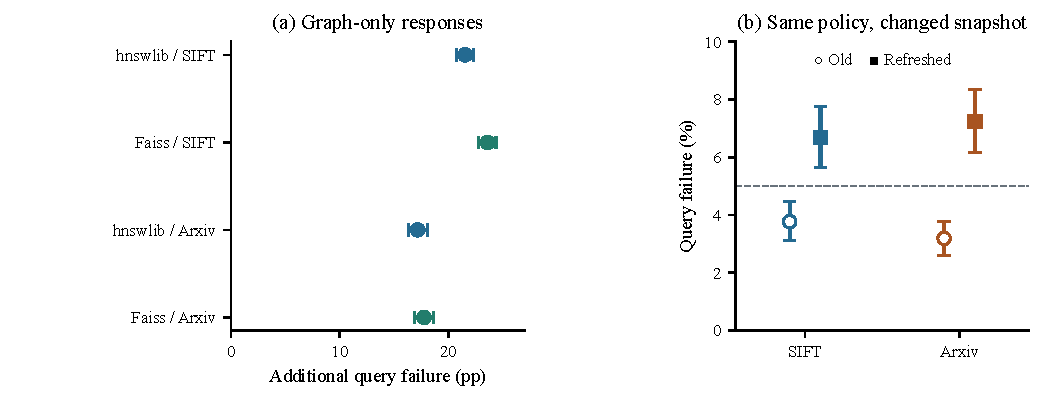
\includegraphics[width=\textwidth]{figures/overview.pdf}
\caption{Two distinct portability tests. Left: graph-only transfer of retrospective first-passing actions; additional failure above each target's own first-passing reference, with 95\% query-cluster intervals conditional on 24 builds. Right: the same executable history-pool policy on matched old and 5\%-refreshed builds; average query risk over ten builds, with crossed target-build/query 95\% intervals. The old/new difference changes both graph and data. Neither comparison treats directed build pairs as independent trials.}
\label{fig:overview}
\Description{Four graph-only incremental-risk estimates are positive. In the separate refresh test, old-policy risk increases on both datasets, crossing the 5 percent line.}
\end{figure*}

\emph{Index-Conditioned Budget Audit} (ICBA) connects these measurements to a serving decision. It identifies the permitted observations, fixes the failure event, isolates policy selection from certification, includes fallback in completed outcomes, and prices information acquisition. Its role is to prevent three distinct quantities from being interchanged: an observed recall improvement, a statistically qualified action, and a net economic benefit.

\emph{Target-calibrated pooling} (TCP) is the recovery case within this audit. It takes historical budgets for the same query, pools them conservatively, and chooses a global grid shift using target-selection queries. The case reveals a useful distinction: the original candidate/fallback procedure uses two individual 95\% bounds, while a post-hoc allocation of a total 5\% confidence-error budget retains fewer candidates. Search savings remain positive under the latter, but Arxiv-Nomic's mean reduction falls from 44.79\% to 29.86\%. Thus the composition of certification has a measurable systems cost.

\begin{table}[t]
\caption*{\textbf{Terms at a glance.} Tables and figures shorten SIFT-100K and Arxiv-Nomic-100K to SIFT and Arxiv.}
\small\begin{tabularx}{\linewidth}{@{}lX@{}}\toprule
Term & Meaning \\\midrule
ICBA & Index-Conditioned Budget Audit: the measurement and decision workflow.\\
TCP & Target-calibrated pooling: the recurring-query history-pool recovery case.\\
NDC & Number of distance calculations; not elapsed time.\\
CP / UCB & Clopper--Pearson / upper confidence bound.\\
Transport risk & Target failure under a transferred action or policy and a declared event.\\
LOTO & Leave one target build out.\\
Unresolved label & No registered action reaches the recall target.\\
Endpoint & Largest grid action, whose risk is measured.\\\bottomrule
\end{tabularx}
\end{table}

We make three contributions. (1) A layered empirical analysis separates graph-only response non-portability, matched refresh-policy deterioration, and external-method qualification. (2) ICBA supplies an executable audit contract and distinguishes fixed-target query certification from build-marginal label coverage. (3) The TCP case quantifies recovery, certification-induced fallback, tails, and the horizon needed to repay acquisition. Vamana-style and Deep1M analyses extend the evidence while retaining their own estimands.

The resulting systems lesson is to version the search policy with the index, query workload, and calibration record. Reusing an action is an operational choice, not a consequence of retaining its parameter name. Target information can recover substantial search efficiency on a recurring workload, but only some targets and serving horizons repay the cost of obtaining it.

\section{Related Work and Positioning}
\label{sec:related}
\sectionaim{Position the rebuild-transfer question without turning heterogeneous methods into a single leaderboard.}

\paragraph{Graph construction and maintenance.}
The final text will connect HNSW and Vamana construction choices to search-path variation. It will distinguish a rebuild of an unchanged vector collection from insert/delete-driven data refresh. Each empirical block must identify which operation it measures before these settings are discussed together.

\paragraph{Adaptive search budgets.}
DARTH, ConANN, ANNiE, and AdaEF are comparison candidates with different input signals, objectives, and execution interfaces. The literature table will record each method's published purpose, query-time information, calibration inputs, and treatment of a new build. A registered bridge is reported as that bridge, with the implementation differences stated. The present W0 numerical snapshot contains DARTH and AdaEF bridge results; it does not supply a newly verified full-method comparison for every named approach.

\paragraph{Risk control and transfer.}
The theory discussion will separate the guarantee for a fixed policy tested on independent queries from the validity of a pipeline that chooses among candidates and fallback actions. Information-theoretic limits explain why source-visible signals can be insufficient under stated observation assumptions. A measured source-to-target gap alone does not establish those assumptions.

\paragraph{Literature completion.}
This W1 section fixes the comparison axes. Bibliographic entries and detailed novelty comparisons will be imported after source and method-identity verification; no unresolved citation is represented as an established reference in this preview.

\section{Portability, Risk, and the Scope of Guarantees}
\label{sec:theory}

\subsection{Execution Risk and Retrospective Responses}
Let $G$ specify a vector snapshot, graph, and search implementation, and let $\mathcal A=(a_1<\cdots<a_J)$ be its native action grid. A policy $\pi$ maps permitted query and history observations to an action. For $q\sim\mathcal Q$,
\begin{equation}
 \begin{aligned}
 Z_G(q,a)&=\indicator\{\rec@k(G,q,a)<\tau\},\\
 \risk_G(\pi)&=\mathbb E_q Z_G(q,\pi(q)).
 \end{aligned}\label{eq:risk}
\end{equation}
Truth is computed against the corresponding snapshot. We distinguish target transport risk $\risk_{G_t}(\pi_s)$, source risk $\risk_{G_s}(\pi_s)$, and a reference-relative increment
\begin{equation}
 \Delta_{s\to t}=\risk_{G_t}(\pi_s)-\risk_{G_t}(\pi_t^{\rm ref}).\label{eq:increment}
\end{equation}
A matched old-to-new comparison instead subtracts $\risk_{G_s}(\pi_s)$, keeping the policy fixed. These two differences answer different questions.

A retrospective first-passing label is $B_G^{\rm first}(q)=\min\{a_j:Z_G(q,a_j)=0\}$. A stable-tail label is
\begin{equation}
 B_G^{\rm tail}(q)=\min\{a_j:Z_G(q,a_\ell)=0\text{ for every }\ell\ge j\}.\label{eq:stable-label}
\end{equation}
Both require query truth; an empty set is $+\infty$, an unresolved label. Native action order need not make either raw recall or realized NDC monotone. Consequently, an action larger than a first-passing label need not succeed, whereas a finite stable-tail label establishes success above it on the recorded grid. The graph-only study uses first-passing labels and evaluates the transferred action's \emph{actual} target response, rather than replacing execution failure by a budget-order comparison.

\subsection{Information Limits Explain What Must Be Observed}
\label{sec:information-limit}
The following classical two-point argument~\cite{yu1997assouad} states why source information alone may be insufficient. For two environments $E_0,E_1$, let $O$ include everything available to the decision rule, with laws $P_0^O,P_1^O$. Suppose acceptable risk--cost decisions form disjoint sets $D_0,D_1$, and loss satisfies $L_i(a)\ge\lambda\indicator\{a\notin D_i\}$ for $\lambda>0$. Then every common decision rule satisfies
\begin{equation}
 \max_i\mathbb E_i L_i(A)\ge\frac{\lambda}{2}\bigl(1-\operatorname{TV}(P_0^O,P_1^O)\bigr).\label{eq:information}
\end{equation}
Indeed, deciding whether $A\in D_0$ defines a test of the environment; its sum of error probabilities is at least $1-\operatorname{TV}$. If a common expensive endpoint is acceptable, disjointness fails and the bound can be vacuous. For random queries, $O$ must include the query jointly with its transcript. Our measurements establish response differences, not an estimate of full-observation total variation or an impossibility result for every policy. The bound explains the information question; the audit below supplies the operational test.

\subsection{Certifying a Fixed-Target Decision}
\label{sec:fixed-cert}
For a policy fixed independently of $n$ i.i.d. target-certification queries, $x$ failures yield the one-sided Clopper--Pearson bound~\cite{clopper1934confidence}
\begin{equation}
 U(x,n;\alpha)=\begin{cases}
 \operatorname{Beta}^{-1}(1-\alpha;x+1,n-x),&x<n,\\1,&x=n.
 \end{cases}\label{eq:cp}
\end{equation}
Acceptance requires $U\le\delta$. Confidence error $\alpha$ and allowed query risk $\delta$ are distinct. At zero failures, $U=1-\alpha^{1/n}$; $\alpha=\delta=0.05$ requires at least 59 queries for acceptance to be possible. With 500 certification queries, nonzero failures can be accepted, but rejection can still reflect limited power near the boundary.

\begin{proposition}[Jointly qualified selection on one target]
\label{prop:simultaneous}
Freeze $K$ policies before certification, and allocate $\alpha_j>0$ with $\sum_{j=1}^K\alpha_j\le\alpha$. On a common i.i.d. certification sample, compute $U_j=U(x_j,n;\alpha_j)$. Select any policy with $U_j\le\delta$, or abstain if none qualifies. Then
\begin{equation}
 \Pr\{\text{a policy is selected and }\risk_G(\pi_{\rm selected})>\delta\}\le\alpha.\label{eq:simultaneous}
\end{equation}
\end{proposition}
\begin{proof}
By a union bound, $\Pr\{\exists j:\risk_G(\pi_j)>U_j\}\le\sum_j\alpha_j$. Otherwise every selectable policy satisfies the risk limit. Independence among policies' bounds is unnecessary.
\end{proof}
This is simultaneous risk control~\cite{angelopoulos2021ltt}. Selection may define the policies using a separate role; the proposition then applies conditionally on selection. A fallback must be included or separately justified. The statement is per fixed target, not simultaneous over a campaign, and does not bound risk conditional on the event of acceptance. The i.i.d. query interpretation concerns the represented workload; fixed-profile replay by itself proves no guarantee for a changed query population.

\subsection{Why Pooling Is Not the Same Certificate}
\label{sec:pooling-theory}
For $m$ source builds and one target with exchangeable budget labels at a fixed query, conformal rank reasoning~\cite{angelopoulos2023conformal} gives a different guarantee. Let $r=\lceil(1-\eta)(m+1)\rceil$. Use the $r$th source order statistic if $r\le m$ and it is finite; otherwise abstain. Then
\begin{equation}
 \Pr\{a(q)<\infty,\ B_t(q)>a(q)\}\le\frac{m+1-r}{m+1}\le\eta.\label{eq:pooling}
\end{equation}
This is build-marginal label coverage for a fixed query. It translates to execution failure for stable-tail labels, but not automatically for first-passing labels. Nine sources offer rank resolution $1/10$, and old/refreshed builds need not be exchangeable. Accordingly, TCP's nine-history replay derives its target qualification from Equation~\eqref{eq:simultaneous}, not from a 5\% conformal claim. The short supplement supplies the rank proof and a margin-based selection result, and states which assumptions are uninstantiated in the experiment.

\section{ICBA and Two Recovery Policies}
\label{sec:auditor}

\subsection{The Audit Contract}
ICBA leaves graph construction and native traversal unchanged. Its input contract names the source and target snapshots, implementation, query population, action grid, permitted observations, failure event, and reference policy. Its output records raw reuse, the selected action, certification counts and bounds, actual fallback, execution risk, and lifecycle cost. These fields also expose when two experimental settings cannot be quantitatively combined.

Target information has three separate uses. Selection chooses a policy using its assigned queries. Certification checks that frozen policy and any fallback; it does not retrain or reorder them. Evaluation measures the completed decision, including fallback executions. A raw-reuse row is retained even if it would fail certification, so a successful endpoint cannot hide an unsuccessful transferred policy. If no policy qualifies, the audit outputs abstention; diagnostic endpoint execution is recorded as unqualified, not approved deployment.

\subsection{TCP: History Pooling Followed by One Target Shift}
\label{sec:tcp-implementation}
The recovery experiment uses native HNSW actions
\begin{equation}
 \mathcal A=(10,20,40,80,120,160,200).\label{eq:tcp-grid}
\end{equation}
For each query and old build, encode the first-passing grid index as $\tilde j_g(q)$; if none passes, store $J$ while retaining the unresolved flag. For target seed $t$, pool the nine old builds other than the matched seed:
\begin{equation}
 j_0^{(t)}(q)=\max_{g\in\mathcal H_t}\tilde j_g(q),\qquad
 \pi_s(q)=a_{\min\{j_0^{(t)}(q)+s,J\}}.\label{eq:shift}
\end{equation}
The same-query old profiles exist for all three target roles. Thus TCP operates on a recurring, profiled workload, not unseen-query budget prediction. Storing a pooled index costs $O(Q)$ for $Q$ profiles; a serving decision is a lookup, addition, and clipping before native search. Acquiring those profiles is a separate, potentially dominant expense.

Target selection scans $s=0,\ldots,J-1$ in ascending order and takes the first shift whose selection-role CP bound at $\alpha=0.05$ is at most 0.05. If none passes, it returns the endpoint shift. This is a selection heuristic, not a multiple-testing certificate or a minimum-NDC optimizer. Both the selected policy and the endpoint are then fixed before certification.

The acronym TCP is retained from the project's history-pooling family; in this paper it denotes the \emph{target-calibrated pooling replay} just defined. Historical artifacts call that family Tiered Conformal Pooling and include a different stable-tail variant at $\tau=0.90$. That variant is not substituted for the first-passing, $\tau=0.95$ results here. The name does not import the exchangeable-build assumptions of Equation~\eqref{eq:pooling}.

\subsection{Original Decisions and a Joint-Error Sensitivity}
\label{sec:tcp-recalibration}
The original replay checks the selected candidate and endpoint separately at $\alpha=0.05$ each. It accepts the candidate if its bound passes, otherwise executes the endpoint with the endpoint's qualification flag. The two allocations sum to 0.10, so they do not provide a 95\% guarantee for the combined selection procedure.

We therefore add a \emph{post-hoc frozen-response sensitivity}: keep every selected shift unchanged, use $\alpha_c=\alpha_e=0.025$, and apply the same candidate-first order. If neither policy passes, abstain. This instantiates Proposition~\ref{prop:simultaneous} at total $\alpha=0.05$ under its query-sampling assumptions, separately for each target. It does not rerun selection, enlarge the action class, or use evaluation to choose a new threshold. Its results are reported alongside the original decisions, not presented as a preregistered replication.

Figure~\ref{fig:workflow} shows the data flow. The audit is reusable independently of TCP: a learned termination rule or a fixed budget can occupy the candidate input, provided its observation contract and failure event are retained.
\begin{figure*}[t]
\centering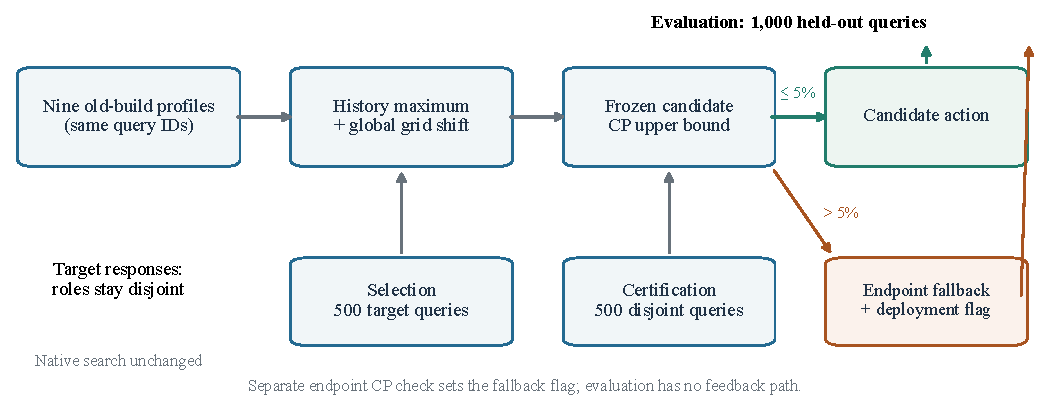
\includegraphics[width=\textwidth]{figures/workflow.pdf}
\caption{ICBA applied to TCP. Same-query old-build profiles define the pooled policy for each target role. Selection chooses one global shift; certification checks the frozen candidate and endpoint; evaluation has no feedback path. The original replay assigns 0.05 to each check. The joint-error sensitivity assigns 0.025 to each, allowing a per-target union bound of 0.05.}
\label{fig:workflow}
\Description{Historical profiles feed an ordered shift selected on 500 queries. A separate 500-query certification role chooses candidate, endpoint, or abstention. Another 1,000 queries evaluate the selected decision.}
\end{figure*}

\subsection{A Source-Certified Slack Bridge}
\label{sec:slack-method}
The second recovery policy removes TCP's target-selection step. For each source build, a source-only design role fixes an action $a_s$. Three registered lanes execute $a_s$ shifted upward by zero, one, or two native grid levels, clipped at the endpoint. On 500 previously untouched source-certification queries, each lane and its endpoint receive error allocations $\alpha_c=\alpha_e=0.025$. A lane is deployable for that source only when both bounds are at most $\delta=0.05$; otherwise it falls back to the certified endpoint. Another 500 untouched queries evaluate the frozen source-to-target decision over all non-diagonal build pairs.

This bridge uses no target selection, target labels, retrospective stable-tail action, or evaluation feedback. The three lanes are separate preregistered estimands rather than a best-after-observation search. Consequently, the experiment can show that a particular fixed slack transfers within a registered implementation family, but not that the lane is uniformly optimal or jointly selected at 95\% confidence across implementations.

\section{Experimental Design and Inference}
\label{sec:methodology}

\paragraph{Graph-only rebuilds.}
Each dataset contains 100,000 base vectors. SIFT-100K uses dimension 128 and Euclidean distance; Arxiv-Nomic-100K uses dimension 768 and normalized inner-product search. Each hnswlib dataset has 24 builds crossing eight seeds and three insertion orders (random, ascending local intrinsic dimensionality, and descending). The clean Faiss replay has 24 registered builds per dataset. Each uses 750 evaluation queries, all 552 non-diagonal directed build pairs, and unchanged base membership and truth. The hnswlib grid is $(10,20,40,80,120,200)$; the Faiss grid is $(16,32,64,128,256,512)$. Their native actions are not equated numerically.

For this study, the source response rule chooses $B_s^{\rm first}(q)$, or the maximum action if unresolved. The target reference chooses $B_t^{\rm first}(q)$ when finite. Its failure is the target-unresolved event; transport failure is either that event or failure of the actual target response at the source-derived action. This convention preserves unresolved mass rather than dropping difficult queries. It is a retrospective response experiment, not a deployable oracle algorithm or an independently source-certified policy.

\paragraph{Refresh and executable-policy replay.}
A separate seed-991 membership change replaces 5\% of each 100K collection with previously excluded vectors, preserving cardinality. Truth is refreshed. Ten old and ten refreshed builds per dataset are replayed through the official DARTH Faiss-HNSW fork, using graph degree parameter $M=16$, construction $ef=100$, one search thread, $k=10$, and Equation~\eqref{eq:tcp-grid}. For each matched pair, TCP excludes that seed from its nine-history pool. The old-to-new diagnostic executes the \emph{same} unshifted policy on both snapshots. Old-side certification checks the pre-existing pooled policy; no source outcome is used to select a different pool.

Target roles contain 500 selection, 500 certification, and 1,000 evaluation queries, with disjoint content and the same IDs reused across builds. Checks against base vectors and insertion reserves accompany the role manifest. Source-history responses for each role precede target selection. Reusing historical profiles for evaluation IDs is part of the recurring-workload contract, not a learned predictor's held-out generalization test. Seeds for graph construction, membership refresh, and statistical resampling are separate roles even where the integer 991 appears in two configurations.

\paragraph{Fresh-query source-only boundary.}
After the preceding analyses were frozen, 1,000 previously untouched query IDs per dataset were split in registered order into 500 source-certification and 500 target-evaluation queries, with zero overlap with the earlier 375-query source-design role or any prior evaluation role. Only these 500/500 roles are prospective. We reuse the same 24 hnswlib and 24 Faiss indexes per dataset; no graph is rebuilt or mutated. The source rule, its 96 actions, the $+0,+1,+2$ lanes, and the role identifiers were sealed before accessing future-query vectors or truth. Candidate and endpoint receive $\alpha=0.025$ each on the source; target evaluation cannot change the action or fallback. Query-bootstrap intervals retain each query's complete 552-direction vector. This stage audits source-only portability conditional on the registered builds.

\paragraph{Post-seal target-certified replication.}
The positive Faiss $+1$ candidate was then fixed without retuning. For each dataset, two additional roles of 500 queries were drawn from a previously unused source-data window and frozen before vector or truth access. They have zero overlap with one another and all earlier registered query roles. On each of 552 directed Faiss pairs, target certification applies $\alpha_c=\alpha_e=0.025$ to the frozen candidate and endpoint; target evaluation uses the other role. The primary 95\% intervals resample the 24 target-build summaries 5,000 times with seed 991. They express variation over the registered target set, not independent pair or query trials. Fixed-machine interleaved timing is reported only as an exploratory sensitivity; NDC remains the primary endpoint.

\paragraph{Metrics.}
Risk is query failure under $k=10$, $\tau=0.95$. Relative serving gain is
\begin{equation}
 g=1-\frac{\bar c_{\rm policy}}{\bar c_{\rm endpoint}},\label{eq:gain}
\end{equation}
a ratio of pooled means, equivalently a relative total-NDC reduction for equal query counts. We report query-pooled p95/p99 NDC and per-target tails, retaining every fallback execution. These are search-work measures, not latency measurements. Observed tail non-increase is distinguished from a formal noninferiority test.

\paragraph{Inference and its sampling units.}
Graph-only intervals resample 750 query IDs, retaining each query's complete directed-pair vector, with builds fixed. They do not treat 552 overlapping directions as independent builds. For the refresh replay we recompute 5,000 crossed bootstrap replicates with seed 991: sample target-build indices, then sample one shared query-index vector used in \emph{all} sampled builds. The paired policy/reference outcomes remain together. Percentile intervals reflect this product resampling, conditional on the stored source histories and selected shifts; they are not confidence guarantees for a new build-generation population. Build-only and shared-query-only sensitivities appear in the supplement.

LOTO deletes a target without refitting, and deletion of the largest relative-gain target is one specified member of that sensitivity family. Acquisition-cost intervals resample target builds conditional on the finite profiling/query records. Vamana and external-method intervals retain their original units, identified beside the corresponding estimates. No interval is pooled across these protocols.

\paragraph{Evidence order.}
We answer nine questions in reading order: graph-only transfer (RQ1), matched refresh transfer (RQ2), audit decisions (RQ3), target-calibrated and fresh-query recovery (RQ4), tails (RQ5), build sensitivity (RQ6), external/family/scale scope (RQ7), economics (RQ8), and reproducibility (RQ9). The old responses and original decisions remain unchanged. Crossed inference, matched-source qualification, joint-error replay, and TCP acquisition accounting are derived analyses of existing records. The source-only boundary and post-seal target-certified replication remain separately labeled and use disjoint fresh roles.

\section{Where Budget Portability Fails}
\label{sec:portability}

\subsection{RQ1: Do Responses Transfer When Only the Graph Changes?}
Retrospective first-passing actions frequently fail after a graph-only rebuild, even though collection membership, queries, and truth are unchanged. Table~\ref{tab:graph-only} reports absolute target risk, the unresolved-reference risk, and their difference. Across hnswlib and Faiss on both datasets, the increment ranges from 17.17 to 23.60 percentage points; every query-cluster interval is above zero. This is a response-level result independent of TCP's pooling or recalibration.

\begin{table*}[t]
\caption{Graph-only response transfer at $k=10$, $\tau=0.95$. Each row has 24 builds, 552 directed pairs, and 750 shared query IDs. Risk entries and increments are percentages or percentage points [95\% query-cluster interval], conditional on the fixed build set. The reference uses the target's own first-passing response; its failures are unresolved queries. Finite variation counts queries with at least two distinct finite first-passing actions, divided by all 750 queries.}
\label{tab:graph-only}
\small\begin{tabular*}{\textwidth}{@{\extracolsep{\fill}}llcccr@{}}\toprule
Implementation & Dataset & Absolute risk [95\% CI] & Reference risk [95\% CI] & Increment [95\% CI] & Finite variation\\\midrule
\GraphOnlyRows
\bottomrule\end{tabular*}
\end{table*}

The variation is principally among finite budgets: 75.87--91.07\% of queries have different finite first-passing actions across builds, while only 0.53--2.67\% switch between resolved and unresolved states. Removing the 1\% of queries with largest incremental contribution leaves increments of 21.37/16.95 percentage points for hnswlib and 23.43/17.53 for Faiss, on SIFT/Arxiv respectively. Endpoint censoring and a handful of extreme queries therefore do not explain the result.

This experiment diagnoses the budget--response relation using retrospective truth on both source and target. It establishes that source success alone is insufficient evidence for action reuse. The measured mechanism is behavioral variation across builds; structural attribution to particular edges or navigation paths lies outside this response-level design.

\subsection{RQ2: Does an Executable Policy Deteriorate after Refresh?}
The matched old/new replay holds the nine-history policy fixed and applies it to both snapshots. Unlike RQ1, this changes 5\% of the vectors as well as rebuilding. SIFT's empirical risk rises from 3.77\% to 6.69\%; Arxiv-Nomic's rises from 3.19\% to 7.24\%. The corresponding paired increments [crossed 95\% interval] are 2.92 [1.75, 4.07] and 4.05 [2.86, 5.31] percentage points. Thus this is a measured deterioration, not merely an absolute target risk with an unknown source baseline.

Independent single-policy CP checks at $\alpha=0.05$ qualify six of ten old SIFT policies and five of ten old Arxiv policies. All eleven fail the corresponding target check. This paired diagnostic uses per-policy checks rather than simultaneous control over the eleven transitions. Target evaluation risk exceeds 5\% in all ten builds of each dataset; removing the highest-risk target leaves 6.61\% and 7.13\%. The deterioration is distributed across targets.

The same policy information is held fixed in each old/new comparison, but the experiment does not separate changed graph paths from changed nearest-neighbor membership. Together, RQ1 and RQ2 establish complementary facts: unchanged data do not make the response function portable, and a recurring-query policy can lose its old qualification after refresh plus rebuilding.

\section{Auditing and Recovering Rebuilt Workloads}
\label{sec:recovery-results}

\subsection{RQ3: What Does the Audit Actually Authorize?}
Auditing unshifted source reuse rejects every candidate and routes all 20 target decisions to the endpoint in the original replay. The audit therefore prevents cheap but unqualified reuse, yet recovers no search saving by itself. Target-selection recalibration changes the candidate before certification. The original procedure accepts 19 of 20 recalibrated candidates; Arxiv seed 1229 has candidate UCB 0.05056 and falls back despite being close to the threshold.

The joint-error sensitivity is more selective (Figure~\ref{fig:decisions}). With $\alpha_c=\alpha_e=0.025$, it accepts all ten SIFT candidates and six Arxiv candidates. All twenty endpoints pass their allocated checks, so four Arxiv decisions fall back and none abstains. The final decision satisfies the per-target construction in Proposition~\ref{prop:simultaneous}, subject to its query-sampling conditions. Certification rejection is not a finding of true unsafety: it changes the supported action given the available 500-query certificate.

\begin{figure*}[t]
\centering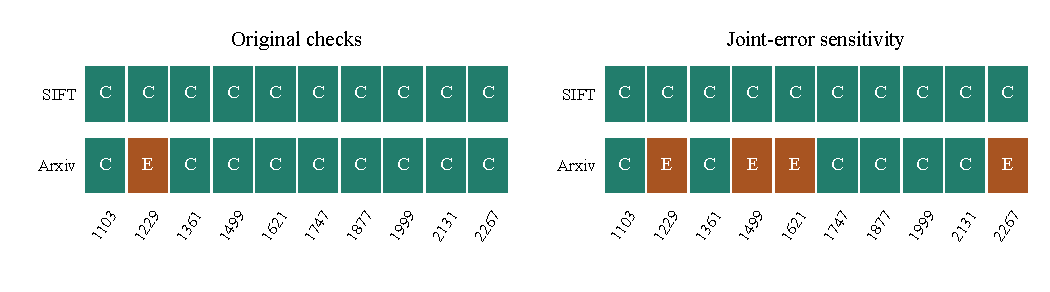
\includegraphics[width=\textwidth]{figures/decisions.pdf}
\caption{One cell per target decision, ordered by registered seed rather than a time axis. C: candidate accepted; E: endpoint fallback. Left: original two individual 95\% checks. Right: post-hoc 0.025+0.025 joint-error allocation. The same selected shifts and certification queries are used in both. Candidate acceptance falls from 19/20 to 16/20, while every completed decision remains qualified by its corresponding endpoint or candidate check.}
\label{fig:decisions}
\Description{SIFT accepts ten candidates under both rules. Arxiv accepts nine under the original rule and six under the joint-error rule; other cells use the endpoint.}
\end{figure*}

\subsection{RQ4: How Much Search Efficiency Is Recovered?}
Recalibration restores substantial search efficiency within the recurring-profile workload (Table~\ref{tab:recovery}). The original decisions reduce risk to 1.79\% and 2.04\%, with relative mean-NDC reductions of 44.39\% and 44.79\%. Crossed resampling widens SIFT's interval compared with the old independently-within-build procedure: it is now [42.76, 46.01]\%, rather than [43.88, 44.91]\%. Preserving shared query dependence changes uncertainty even when the point estimate is unchanged.

\begin{table*}[t]
\caption{Completed refresh decisions on ten targets and 1,000 evaluation queries per target. Query risk and relative mean-NDC reduction are percentages [crossed 95\% interval]; intervals are conditional on fixed source histories and selected shifts. Original and joint-error rows differ only in certification composition. All fallback executions are included. Mean and p95/p99 are distance calculations, not latency.}
\label{tab:recovery}
\small\begin{tabular*}{\textwidth}{@{\extracolsep{\fill}}llrrrrr@{}}\toprule
Dataset & Decision & Risk [95\% interval] & Reduction [95\% interval] & Mean NDC & p95 & p99\\\midrule
\RecoveryRows
\bottomrule\end{tabular*}
\end{table*}

Under the joint-error allocation, SIFT is unchanged, while Arxiv risk becomes 1.68\% and relative mean-NDC reduction becomes 29.86 [14.75, 45.00]\%. Figure~\ref{fig:tradeoff} shows that stricter qualification moves the decision toward the endpoint: it reduces risk and sacrifices some efficiency. The positive intervals support recovery of useful search work on both datasets, not a claim of optimality over adaptive-search methods with different information budgets. In particular, the comparator here is the same graph's fixed endpoint, not the best target-trained method.

\begin{figure}[t]
\centering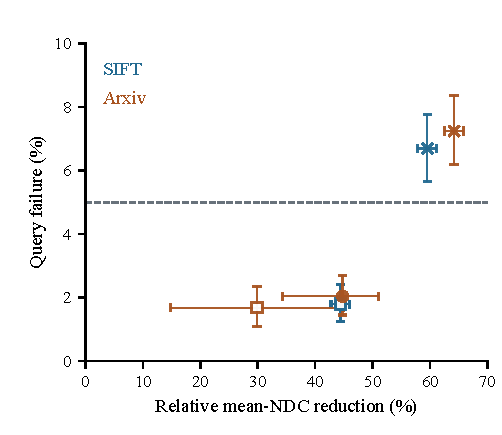
\includegraphics[width=\linewidth]{figures/tradeoff.pdf}
\caption{Refresh risk--work tradeoff with crossed 95\% intervals. The 5\% line is the query-risk target, not a confidence bound. Filled symbols: original recalibration; open symbols: joint-error replay; crosses: direct reuse. SIFT's original and joint points coincide.}
\label{fig:tradeoff}
\Description{Direct reuse has larger search savings but more than 5 percent failure. Both recalibration rules have lower risk; the joint Arxiv point gives up some work saving.}
\end{figure}

\subsection{RQ4 Boundary and Replication: Can Fixed Slack Transfer?}
\label{sec:fresh-bridge}
The first fresh-query stage tests the source-derived policy of Section~\ref{sec:slack-method}, not TCP. Source certification and 500 held-out target queries are different objects: the former determines the executable candidate, while the latter initially supplies a portability audit rather than a target deployment certificate. The complete three-lane table remains in the supplement. Its main boundary is simple. On hnswlib, the $+1$ lane clips to the endpoint for all registered sources and therefore saves no work on either dataset. On Faiss, the same lane retains 8.27\% and 29.09\% mean-NDC savings, with held-out empirical risks of 0.18\% and 0.67\%; no held-out direction exceeds 5\% empirical risk. This stage fixes a viable candidate family but does not authorize target deployment.

The post-seal replication closes that gap with new, mutually exclusive target certification and evaluation roles (Table~\ref{tab:target-certified}). Every candidate and endpoint has a target CP UCB below 5\%; all 552 directions per dataset deploy the frozen candidate, with no fallback or abstention. The largest candidate certificate counts are 5/500 on SIFT and 6/500 on Arxiv-Nomic (UCBs 2.32\% and 2.59\%). Evaluation risk is 0.126 [0.040, 0.250]\% on SIFT and 0.530 [0.233, 0.915]\% on Arxiv-Nomic. Mean-NDC savings remain 8.283 [7.921, 8.557]\% and 29.083 [28.653, 29.518]\%. These crossed target--query intervals are wider than the target-only intervals but leave the conclusions unchanged. Pooled and worst-target p95 ratios remain below one, and leaving out any target preserves positive mean savings.

\begin{table*}[t]
\caption{Post-seal Faiss target-certified replication. Each dataset has 24 targets, 552 directed decisions, 500 target-certification queries, and 500 disjoint evaluation queries. C/F/A counts candidate, fallback, and abstention decisions. Risk and mean-NDC saving are percentages [95\% crossed target-build/query-ID bootstrap interval]. P95 reports pooled/worst-target ratios to the endpoint; LOTO is the minimum mean saving after deleting one target.}
\label{tab:target-certified}
\small\begin{tabular*}{\textwidth}{@{\extracolsep{\fill}}lrrrrr@{}}\toprule
Dataset & C/F/A & Eval. risk [95\% CI] & NDC saving [95\% CI] & P95 ratio & LOTO saving\\\midrule
\TargetCertifiedRows
\bottomrule\end{tabular*}
\end{table*}

The candidate is below the endpoint in 92/552 SIFT directions and 322/552 Arxiv directions; in the others the upward rung clips to the endpoint. This explains why every decision can deploy the candidate while many isolated directions have zero saving. It also preserves the implementation boundary: no target-certified hnswlib claim is made because the registered hnswlib candidate already equals the endpoint. Fixed-machine interleaved timing points in the same direction (9.27\% and 26.57\% mean reductions), but remains exploratory; NDC is the primary efficiency endpoint.

\subsection{RQ5: Does Recovery Worsen the Search-Work Tail?}
Neither recalibration rule increases query-pooled p95 or p99 relative to the endpoint. For joint-error replay, p95 is 2,349 versus 2,615 NDC on SIFT, and 3,117 versus 3,252 on Arxiv; p99 is 2,774 versus 2,855 and 3,460 versus 3,504. Every individual target also has non-increasing p95 and p99. Figure~\ref{fig:tails} displays the per-target ratios without connecting unrelated seeds.

\begin{figure}[t]
\centering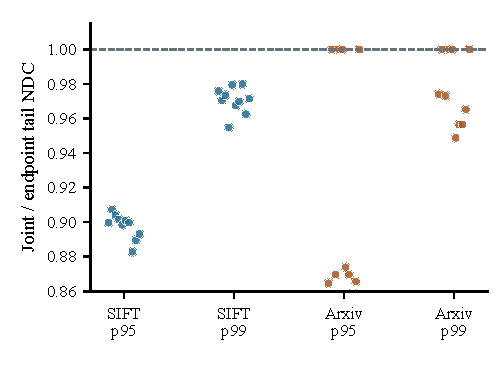
\includegraphics[width=\linewidth]{figures/tails.pdf}
\caption{Per-target tail ratios for joint-error replay, relative to that target's endpoint; ten dots per dataset/quantile. Equality reflects an endpoint fallback. All ratios are at most one. These descriptive tail comparisons are not formal noninferiority certificates or wall-clock results.}
\label{fig:tails}
\Description{Paired target p95 and p99 ratios fall at or below the equality line; endpoint fallback targets have ratio one.}
\end{figure}

The fallback is a build-level choice, so its serving distribution is exactly the fixed endpoint's distribution for that build. Combining it with candidate-serving builds can change pooled quantiles even without changing a candidate's query path. Reporting both pooled and per-target tails avoids hiding this composition effect. It also avoids inferring tail behavior from the much larger mean gain alone.

\subsection{RQ6: Is the Benefit Driven by One Target?}
The minimum LOTO mean-NDC reduction is 44.37\%/44.23\% for original SIFT/Arxiv decisions, and 44.37\%/27.64\% for joint-error decisions. Deleting the largest relative-gain build produces those same minima in these records. These are overlapping checks, not independent confirmations. Target-only and shared-query-only interval sensitivities in the supplement show different uncertainty sources: SIFT's variation is dominated by queries, whereas Arxiv's stricter-rule result also varies strongly with the candidate/fallback choice across targets. The retained positive direction supports a fixed-target-set recovery finding; it does not certify an unseen rebuild distribution.

\section{RQ7: Scope across Methods, Scale, and Graph Family}
\label{sec:families}

\paragraph{External adaptive methods.}
The frozen DARTH adapters produce target query-failure rates of 22.55\% on SIFT-100K and 23.12\% on Arxiv-Nomic-100K at $\rec@10<0.95$. Ada-ef yields 9.52 [9.44, 9.60]\% on ten Arxiv targets, with a target-build bootstrap conditional on its query set. All ten Ada-ef candidate certificates fail; audited execution uses the qualified endpoint and has zero search gain relative to that endpoint. Ada-ef is absent from Euclidean SIFT because the inspected estimator implements cosine/inner-product semantics, not a semantics-preserving L2 path. Its exclusion is an implementation-scope boundary, not a failed SIFT result.

These measurements show why query-risk qualification matters beyond TCP. They do not, without matched source checks, identify how much failure was caused by rebuilding, and the event is not interchangeable with mean recall or expected false-negative fraction. They therefore remain qualification studies rather than a ranking of published methods. The TCP comparator and information budget are stated separately.

\paragraph{Larger scale.}
On Deep1M, eight hnswlib builds cross four seeds with two insertion orders, giving 56 directed pairs on 1,000 queries. Source-derived first-passing actions have 28.86\% transport risk against 8.82\% target-reference risk. The incremental risk is 20.04 [17.29, 22.77] percentage points, using a target-build bootstrap conditional on the frozen source histories and query set. Keeping the reference risk visible matters: this is additional loss above a difficult, partly unresolved target reference, not a transfer from a zero-risk baseline.

A preregistered replication reuses the eight indexes with disjoint 500/500/500-query roles. All 56 non-clipped candidates pass target certification; evaluation risk is 1.63 [0.80, 2.61]\% and mean-NDC saving versus efSearch 1200 is 34.28 [33.53, 35.05]\%. Every target and leave-one-target-out analysis remains positive; this is scale, not cross-family, confirmation.

\paragraph{Vamana-style evidence.}
Six source and six separate target builds produce 36 directions and 750 queries per dataset, using native search-list size and beam width one. The frozen event table combines its stage-specific under-budget and censoring outcomes. A target-build reanalysis gives 16.86 [15.88, 17.93]\% on SIFT and 11.37 [10.80, 11.99]\% on Arxiv. Its recorded responses do not reconstruct exactly the first-passing execution estimand used for hnswlib/Faiss. We retain it as directional cross-family evidence, not another row of Table~\ref{tab:graph-only}.

Vamana cost-tax intervals include zero: 1.07 [$-1.03$, 2.86]\% and 1.17 [$-0.83$, 3.03]\%, respectively, for the mean of per-target ratios in that reanalysis. Thus it supplies no established positive cost penalty or cross-engine superiority. Table~\ref{tab:scope} summarizes which question each setting can answer.

\begin{table*}[t]
\caption{Scope of the extension evidence. Each row retains its event, reference, and inference unit. All numeric intervals in the text are 95\%; no common cross-engine ranking or pooled effect is formed.}
\label{tab:scope}
\small\begin{tabularx}{\textwidth}{@{}lXXl@{}}\toprule
Setting & Event and reference & Supported comparison & Unit / query count\\\midrule
DARTH & Absolute target $\rec@10<0.95$ risk; no matched reference subtraction & Target qualification under the frozen adapter & Target summaries; 1,000/build\\
Ada-ef & Absolute target $\rec@10<0.95$ risk; endpoint for audited saving & Candidate rejection versus endpoint execution on Arxiv & 10 target builds; 1,000/build\\
Deep1M & Transport versus target reference; certified slack versus efSearch 1200 & Transfer loss and certified recovery at 1M scale & 8 targets; 1,000 prior + 1,500 fresh\\
Vamana-style & Frozen stage under-budget/censoring event; stage-specific cost reference & Directional cross-family transfer evidence, not a harmonized HNSW increment & 6 target builds; 750 shared queries\\\bottomrule
\end{tabularx}
\end{table*}

Together with RQ1, these results support a layered conclusion: response non-portability is seen across HNSW implementations and at larger scale; qualification of adaptive actions is operationally consequential; and a distinct graph family supplies supporting evidence with narrower semantic comparability. They do not establish uniform failure across every graph family or every adaptive policy.

\section{RQ8: When Does Recovery Repay Its Information Cost?}
\label{sec:recovery}

Search savings repay recovery only over a sufficiently long recurring workload. We express the accounting in native distance evaluations,
\begin{equation}
 C_\pi(N)=C_{{\rm acquire},\pi}+N\bar c_\pi,\qquad
 N_{\rm BE}=\frac{\Delta C_{\rm acquire}}{\bar c_{\rm end}-\bar c_\pi}.\label{eq:breakeven}
\end{equation}
If incremental acquisition is positive but serving saving is not, no finite break-even exists. Graph rebuilding is common to both policies on the same target. Control adds no distance calls but is not assigned zero elapsed time.

\paragraph{Two explicit acquisition scenarios.}
With \emph{cached history}, old query profiles and their truth are sunk costs. We charge the complete target-selection grid, the selected candidate's certification searches, additional endpoint-certification searches where the actions differ, and exact target truth for the 1,000 selection/certification queries. Truth is modeled as one scan of 100,000 vectors per query. With \emph{cold complete history}, we also charge sequential old-build profiling for all three roles on all nine contributing histories and exact old-snapshot truth for all 2,000 query IDs. That truth is reusable across old builds of the same collection and is counted once, not nine times. These are workload-acquisition scenarios, not newly measured elapsed-time costs.

We conservatively charge all endpoint certification to recovery, although the reference may also need some of this work. We price the evaluated decision rule without charging repeated calls for the same action and query twice. The earlier partial calculation included old profiling only for evaluation IDs and omitted old truth and extra endpoint certification. Completing these items materially changes the economic conclusion.

\begin{table}[t]
\caption{Joint-error recovery: break-even query executions in thousands [95\% target-build interval], conditional on the finite acquisition workload. The ratio of mean overhead to mean saving is not a per-build guarantee. ``No saving'' counts nonamortizing targets.}
\label{tab:economics}
\small\begin{tabular*}{\linewidth}{@{\extracolsep{\fill}}llrr@{}}\toprule
Dataset & History & Break-even, $10^3$ & No saving\\\midrule
\CostRows
\bottomrule\end{tabular*}
\end{table}

For joint-error replay, cold-history break-even is approximately 396,000 executions on SIFT and 457,000 on Arxiv, versus 129,000 and 148,000 with cached history (Table~\ref{tab:economics}). Four Arxiv targets fall back and never repay a positive recovery overhead through serving savings. The original procedure has lower cold-history break-even on Arxiv, approximately 305,000, but different certification composition. It is therefore insufficient to attach the original economics to the stricter decision rule.

At $N=10^6$, the cold-history joint-error model yields mean net savings of about 490 million NDC on SIFT and 389 million on Arxiv. Their target-build intervals are [488, 491] million and [31, 747] million, respectively. At $10^5$, both cold-history means are negative. Figure~\ref{fig:cost} shows how the crossover depends on what information already exists.

\paragraph{Target-certified fresh-query policy.}
The post-seal replication has a different ledger. Per dataset, the same 500 certification queries are run on every target and reused across its 23 source histories. For each target, exact truth costs $500\times100{,}000$ distances; measured candidate and endpoint searches are added with identical actions deduplicated. Pairwise accounting charges this target audit to every directed source--target unit, whereas shared-target accounting charges it once and reuses it over the 23 registered sources (Table~\ref{tab:target-stage-cost}). On evaluation, mean candidate/endpoint work is 9,169.58/9,997.70 NDC on SIFT and 8,234.58/11,611.52 on Arxiv, yielding the 8.283\% and 29.083\% reductions in Table~\ref{tab:target-certified}. For example, SIFT pairwise acquisition sums to 30.588 billion NDC and serving saving to 457,122.72 NDC per portfolio execution, giving $30.588\text{B}/457{,}122.72=66{,}914$ executions. Shared-target acquisition is 1.380 billion NDC over the same serving saving, giving 3,019 executions. The pairwise/shared acquisition ratio is 22.17 rather than 23 because the shared audit evaluates the union of distinct candidate and endpoint actions for a target, whereas each pairwise audit evaluates only the actions required by that direction. The corresponding Arxiv thresholds are 17,018 and 755. Because clipping gives zero saving in 460/552 and 230/552 directions, the pairwise ratios are portfolio thresholds, not per-direction guarantees.

\begin{table*}[!t]
\caption{Target-stage NDC ledger for the target-certified Faiss candidate. Break-even is a ratio of summed acquisition cost and serving saving [95\% target-build bootstrap interval]. ``No saving'' counts units with zero serving reduction; the final column is the first registered horizon with positive aggregate net NDC.}
\label{tab:target-stage-cost}
\small\begin{tabular*}{\textwidth}{@{\extracolsep{\fill}}llrrrr@{}}\toprule
Dataset & Accounting & Units & Break-even [95\% CI] & No saving & First positive $N$\\\midrule
\TargetStageCostRows
\bottomrule\end{tabular*}
\end{table*}

At $N=10^6$ per direction, mean shared-target net saving per target (aggregated over its 23 source directions) is 18.99 billion NDC on SIFT and 77.61 billion on Arxiv; both target-build interval lower bounds, LOTO minima, and delete-largest-target checks remain positive. This closes the \emph{target-stage} NDC ledger. It does not close complete cold lifecycle economics: historical source-policy acquisition has no compatible per-query NDC record and is not assigned zero. Exact-truth/control wall time is also absent, so search-only timing break-even remains diagnostic rather than an end-to-end latency result.

\begin{figure}[t]
\centering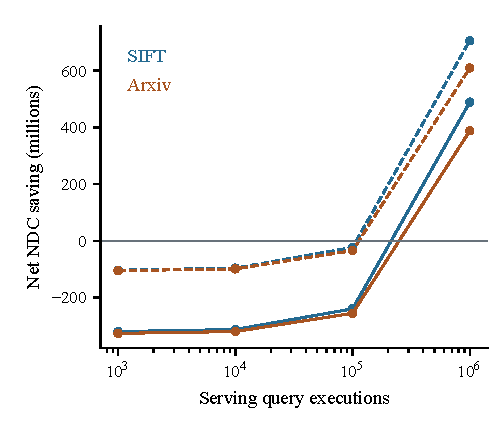
\includegraphics[width=\linewidth]{figures/cost.pdf}
\caption{Joint-error recovery, modeled net distance savings per target versus serving horizon. Solid: cold complete history; dashed: cached history. Dots mark reported horizons; lines depict the stated affine cost model, not additional measurements. Endpoint-fallback targets remain in the average.}
\label{fig:cost}
\Description{Net savings are negative for short horizons and positive at one million executions. Cold-history accounting crosses zero later than cached-history accounting.}
\end{figure}

This calculation assumes repeated executions over the profiled workload. A cache miss requires new information or a declared endpoint action; an unbounded stream of new query identities can invalidate the amortization. Acquisition of historical graphs themselves is not reconstructed here: cold history means acquiring profiles on retained graphs, not rebuilding the entire archive. Memory traffic, storage, energy, and control time require separate prices. The result is a conditional distance-work benefit, not an end-to-end latency or monetary claim.

\section{Reproducibility and Operational Implications}
\label{sec:discussion}

\subsection{RQ9: Can the Decisions and Numbers Be Checked?}
The compact evidence package contains per-target certification failures, both confidence allocations, selected shifts, paired evaluation arrays, cost components, the fresh-query summary, and generated table inputs. One script regenerates figures and typeset rows; another reanalyzes frozen native-response files through explicit repository and replay-root arguments. It checks the original twenty target decisions before deriving the new sensitivities. Historical records and the prospective source-slack stage remain separately labeled.

The preceding artifact audit preserved 80 pre-audit scientific files, passed a neutral-path smoke and 28 focused tests, and exposed guarded replay entry points for DARTH, Vamana, and Deep1M. In a clean Python environment built from the anonymous allowlist alone, the manuscript package passes 244 earlier evidence checks, reproduces all generated table text exactly, regenerates six figures, and verifies 210/210 source-only fresh-query checks. The post-seal checker additionally validates all 1,104 target decisions, 48 target summaries, four cost summaries, and both cost ledgers. It includes sanitized registration records for both fresh-query stages. These are reference-environment checks, not independent native-search replication. Recreating native searches still requires separately provisioned vectors, truth, indexes, binaries, and role manifests. The supplement gives the statistical recipes and detailed certificate tables; the package maps each claim to its compact evidence source.

\paragraph{Interpretation for index maintenance.}
The experiments suggest three operator decisions. After a graph-only rebuild, a historical budget is evidence about a source response, not the new one. After refresh, test the unchanged policy on the target rather than interpreting high mean recall as query-risk qualification. If recovery is considered, evaluate its completed candidate/fallback procedure and the horizon needed to pay for information. ICBA makes these checks explicit; TCP demonstrates target-calibrated recovery on a recurring workload, while the fresh-query bridge separates low-cost source candidate construction from target qualification.

\paragraph{Remaining boundaries.}
The graph-only result is a retrospective response diagnostic; TCP's positive evidence is a Faiss-HNSW recurring-profile case on two 100K datasets. The source-only boundary is prospective only for its original 500/500 roles. The post-seal replication uses new 500/500 target roles, remains conditional on 24 registered Faiss builds, and does not establish cross-implementation recovery. Its target-stage NDC ledger is complete, but its historical source-acquisition and full wall-clock ledgers are not estimable. Deep1M extends response evidence, not recovery economics. The TCP certification sensitivity is post-hoc and per target. The experiments do not identify a causal navigation-edge mechanism, demonstrate a learned unseen-query predictor, or establish hardware-general latency gains. Dynamic graph repair and target-trained adaptive methods are alternatives, not defeated baselines.

\section{Conclusion}
Search budgets are part of an index's operational state. On unchanged collections, source-derived first-passing actions incur substantial additional failure across hnswlib and Faiss rebuilds. After refresh, an unchanged recurring-query policy deteriorates and TCP recovers useful work on a recurring-query population. On fresh queries, a simpler source-derived slack rule retains work only on the registered Faiss grids; a post-seal replication then shows that the fixed Faiss candidate can be target-certified without losing its mean or tail benefit. ICBA makes these outcomes comparable without conflating them: certification, serving-work savings, target-stage amortization, and complete lifecycle value remain distinct. Each must be decided for the target index, implementation, action grid, and workload.

\balance
\bibliographystyle{ACM-Reference-Format}
\bibliography{references}
\end{document}
